% Appendix A

\chapter{Interfáz y programas del instrumento de calibración} % Main appendix title

\label{AppendixB} % For referencing this appendix elsewhere, use \ref{AppendixA}

\lhead{Appendix B. \emph{ Interfáz y programas del instrumento de calibración.}} % This is for the header on each page - perhaps a shortened title

\graphicspath{{Figures/planos_piezas_rotador/}{../Figures/planos_piezas_rotador/}} 

En este Anexo se presentan los programas por medio de los cuales se
utiliza el instrumento de caracterización de SLMs. 
\section{Interfaz de calibración de motores}
Antes derealizar la caracterización de un SLM es necesario calibrar y poner a punto los
rotadores de elementos ópticos. Esto implica ajustar el elemento
óptico sobre el buje de cada rotador. Como no hay 
ninguna garantía de que los ejes rápidos de los retardadores y polarizadores hallan
quedado alineados con la posición cero de su rotador respectivo, se
ubica un polarizador antes de la cámara en posición vertical como
analizador y se realiza una
calibración de cada rotador en la cual el instrumento rota el elemento óptico hasta
encontrar un mínimo de intensidad y reinicializa el contador de pasos
del motor. Luego se procede a medir la cantidad de
pasos por vuelta de cada motor para saber la relación entre pasos y
grados de rotación que es esencial para establecer un PSG o PSD
determinado.

La Fig. \ref{fig:polarizer_calib} muestra un recorte de
pantalla del instrumento de calibración de motores y cada una de sus secciones.
\begin{figure}
\centering
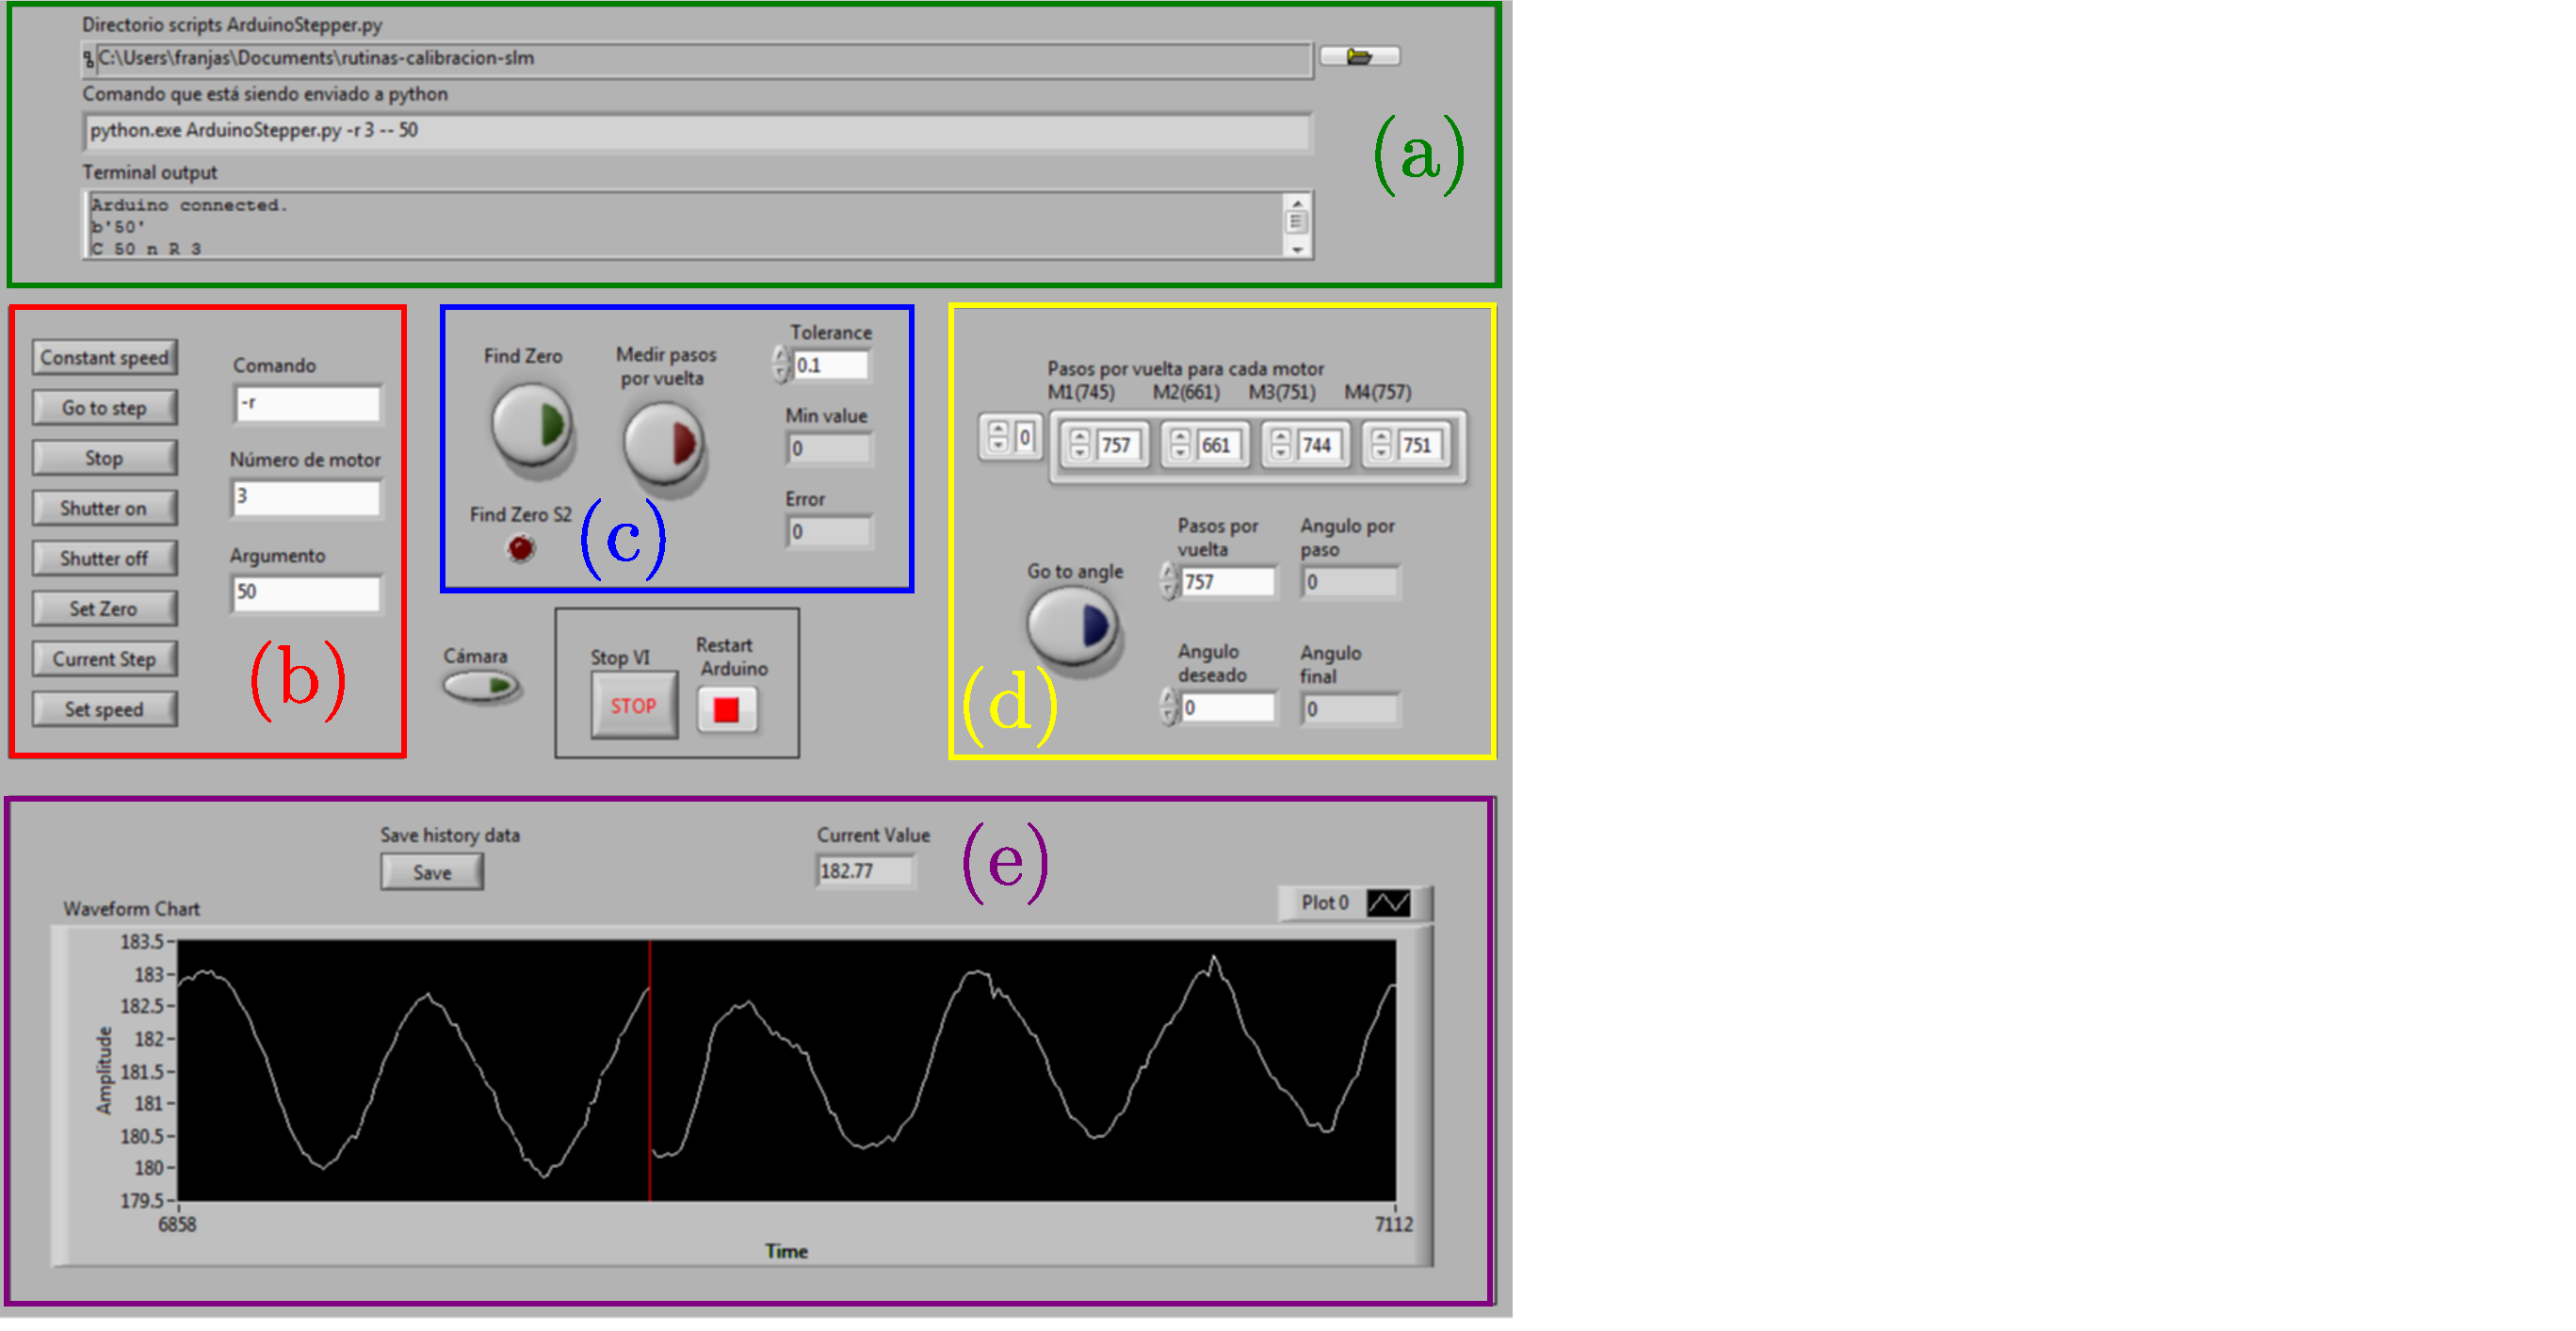
\includegraphics[scale = .5]{polarizer_calib.pdf} 
\caption[Interfaz del programa para calibración de
motores.]{Instrumento virtual para calibración de rotadores. (a)
  Directorios donde se aloja la rutina de comunicación serial e
  información envíada, (b) panel de control para usar cáda función de
  los rotadores, y (c) botones para encontrar el cero de un rotador y
  para medir pasos por vuelta. (d) Permite específicar los pasos por
  vuelta de cada rotador, y enviar un rotador dado a una posición
  deseada y (e) permite visualizar la evolución de la intensidad
  medida por la cámara. }
\label{fig:polarizer_calib}
\end{figure}
En el recuadro (a) del instrumento se encuentra la dirección del
directorio en el cual está alojada la librería de comunicación serial
(copiada en la sección \ref{sec:python_serial})
que envía los comandos al Arduino. Adicionalmente se muestran, en dos
recuadros, los comandos seriales que están siendo enviados a la
terminal de python, y los que están siendo retornados como respuesta.
Luego, en el recuadro (b) hay botones para cada una de las acciones que
se pueden ejecutar sobre un motor dado, y se incluyen dos botones que
controlan un obtulador que también es activado por el
instrumento. Las casillas de esta sección 
permiten definir el número del motor al cual se está enviando el
comando y el argumento asociado si aplica. En el caso que quedó
registrado se estaba enviando la orden de movimiento continuo a una
velocidad de 50 pasos por minuto al motor 3. Esta sección del instrumento es útil para
controlar de forma manual los motores y hacer pruebas de calibración
fina. A diferencia de la anterior, la sección (c) permite hacer
medidas automatizadas que implican una sucesión de ordenes sobre un
motor en particular. El botón de la izquierda permite medir el cero de
un rotador una vez se a ajustado el elemento óptico, y el botón de la
derecha mide la distancia entre dos ceros para determinar el número de
pasos que se necesita mover el motor para completar una rotación de
$360^{\circ}$. Las casillas superior permite definir la
tolerancia que se usa para determinar cuando se ha llegado a un valle,
y las otras dos retornan el valor mínimo sensado y el error obtenido. 
La sección (d) del instrumento se usa una vez son conocidos los pasos
por vuelta de cada motor y simplemente permite mover los rotadores
usando ángulos y no pasos como argumento de entrada. Finalmente, la
sección (e) contiene una gráfica que actúa como indicador e historial
de la intensidad promedio medida por la cámara CCD. Este indicador
permite confirmar que efectivamente cada rotador ha sido alineado
con respecto al cero de su elemento óptico. 

\section{Interfaz para toma de medidas}

El instrumento para toma de medidas integra las rutinas de movimiento
de rotadores mencionadas en la sección anterior con los algoritmos de
medida de modulación implementados en Matlab para automatizar la
medida de múltiples estados. Siendo así es un instrumento virtual con
múltiples pestañas y aplicaciones que permiten tanto un contról
fino para medidas y observaciones simples como funciones para automatización y la
toma de conjuntos de medidas. 

En las Fig. \ref{fig:SLM_calib} y \ref{fig:SLM_calib2} se muestran
casi todas las pestañas y recuadros del instrumento virtual para tomas
de medidas. De forma similar al instrumento anterior, la pestaña de directorios
\ref{fig:SLM_calib}(a) permite al usuario especificar los directorios
en los cuales se han almacenado los archivos para comunicación serial
escritos en Python y los de adquisición de curvas de modulación
escritos en Matlab. En esta misma sección se puede seleccionar el
archivo .txt que contiene la lista de medidas a realizar en un proceso
automatizado de medida. El contenido de dicho archivo es una lista de
configuraciones de polarizador y retardadores que generan todos los
PSG y PSD. 
% Un archivo para medir las primeras 10 combinaciones de la
% notación de la Fig. \ref{fig:braket_100_notation} sería el siguiente:
% \begin{lstlisting}
% 0	0	90	0
% 0	0	90	90
% 0	0	0	45
% 0	0	90	45
% 0	0	-45	45
% 0	0	45	-45
% 0	0	0	67.5
% 0	0	90	22.5
% 0	0	-45	22.5
% 0	0	-45	-67.5
% \end{lstlisting}
El recuadro \ref{fig:SLM_calib}(b) muestra la pestaña en la cual se
encuentra el botón para ejecutar el conjunto de medidas listadas en el
archivo mencionado anteriormente. Adicionalmente, ésta contiene una casilla
para escribir el nombre del archivo de salida que contiene las curvas
de modulación para cada medida, y 4 casillas de lectura que indican
el ángulo actual de cada rotador. El recuadro \ref{fig:SLM_calib}(c)
resalta la pestaña que contiene la ventana para visualizar las
imágenes adquiridas por la cámara, y el recuadro
\ref{fig:SLM_calib}(d) es un inserto del instrumento para controlar
rotadores. La ventana de visualización es de particular interés para
observar y calibrar los patrones de franjas en medidas de modulación
de fase.
\begin{figure}
\centering
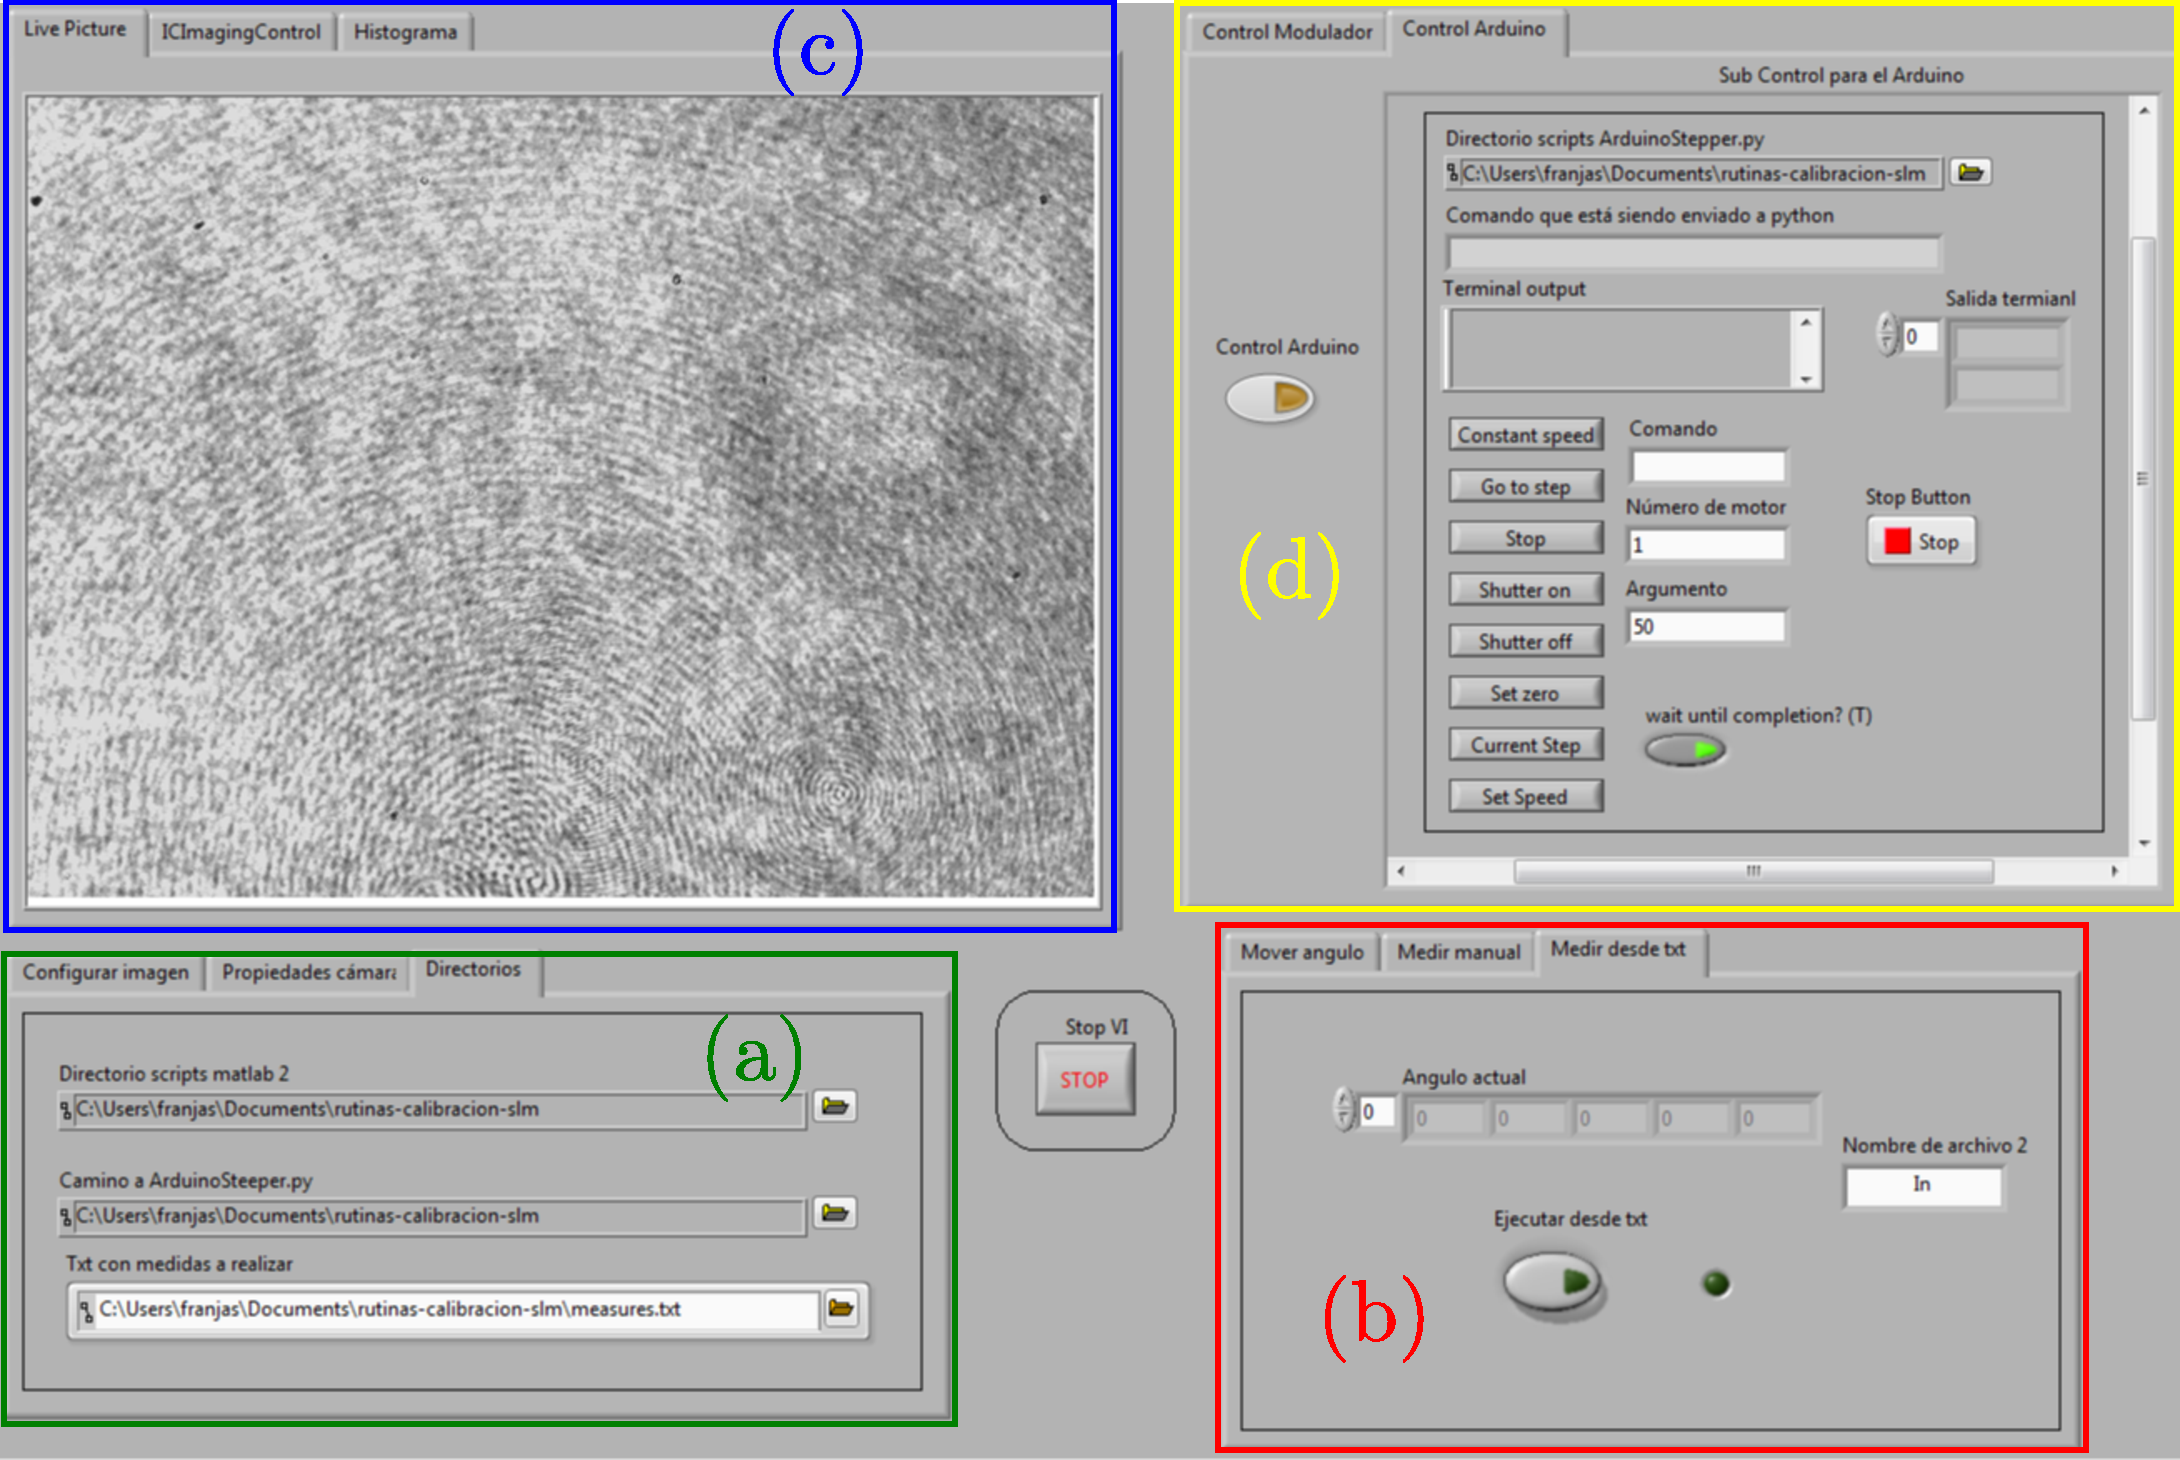
\includegraphics[scale = .4]{SLM_calib.pdf} 
\caption[Interfaz del programa para toma de medidas 1.]{Instrumento
  virtual para toma de medidas. (a) Directorios donde se alojan las rutinas de comunicación serial, y
  de medición de modulación, así como los archivos .txt con la lista
  de combinaciones de PSG y PSD. (b) Sección para ejecutar un conjunto de
  medidas de forma automatizada. (c) Monitor que muestra las imagenes
  detectadas por la cámara, y (d) panel de control para usar cada función de
  los rotadores.}
\label{fig:SLM_calib}
\end{figure}

Por otra parte, el recuadro \ref{fig:SLM_calib2}(a) contiene los
botones usados para la configuración de propiedades de la cámara como
ganancia, brillo y tiempo de exposición. La pestaña de
\ref{fig:SLM_calib2}(b) tiene botones y casillas que permiten medir
curvas de modulación de amplitud y fase de forma manual y a diferencia
de la pestaña \ref{fig:SLM_calib}(b) en ésta se pueden especificar los
ángulos de cada rotador para una medida específica sin necesidad de
cargar un archivo de texto. Finalmente, el recuadro
\ref{fig:SLM_calib2}(c) contiene un deslizador que permite proyectar
al SLM una imagen con dos rectángulos, uno homogéneo con nivel de gris constante como
referencia y otro con diferentes valores de gris.  
\begin{figure}[h!]
\centering
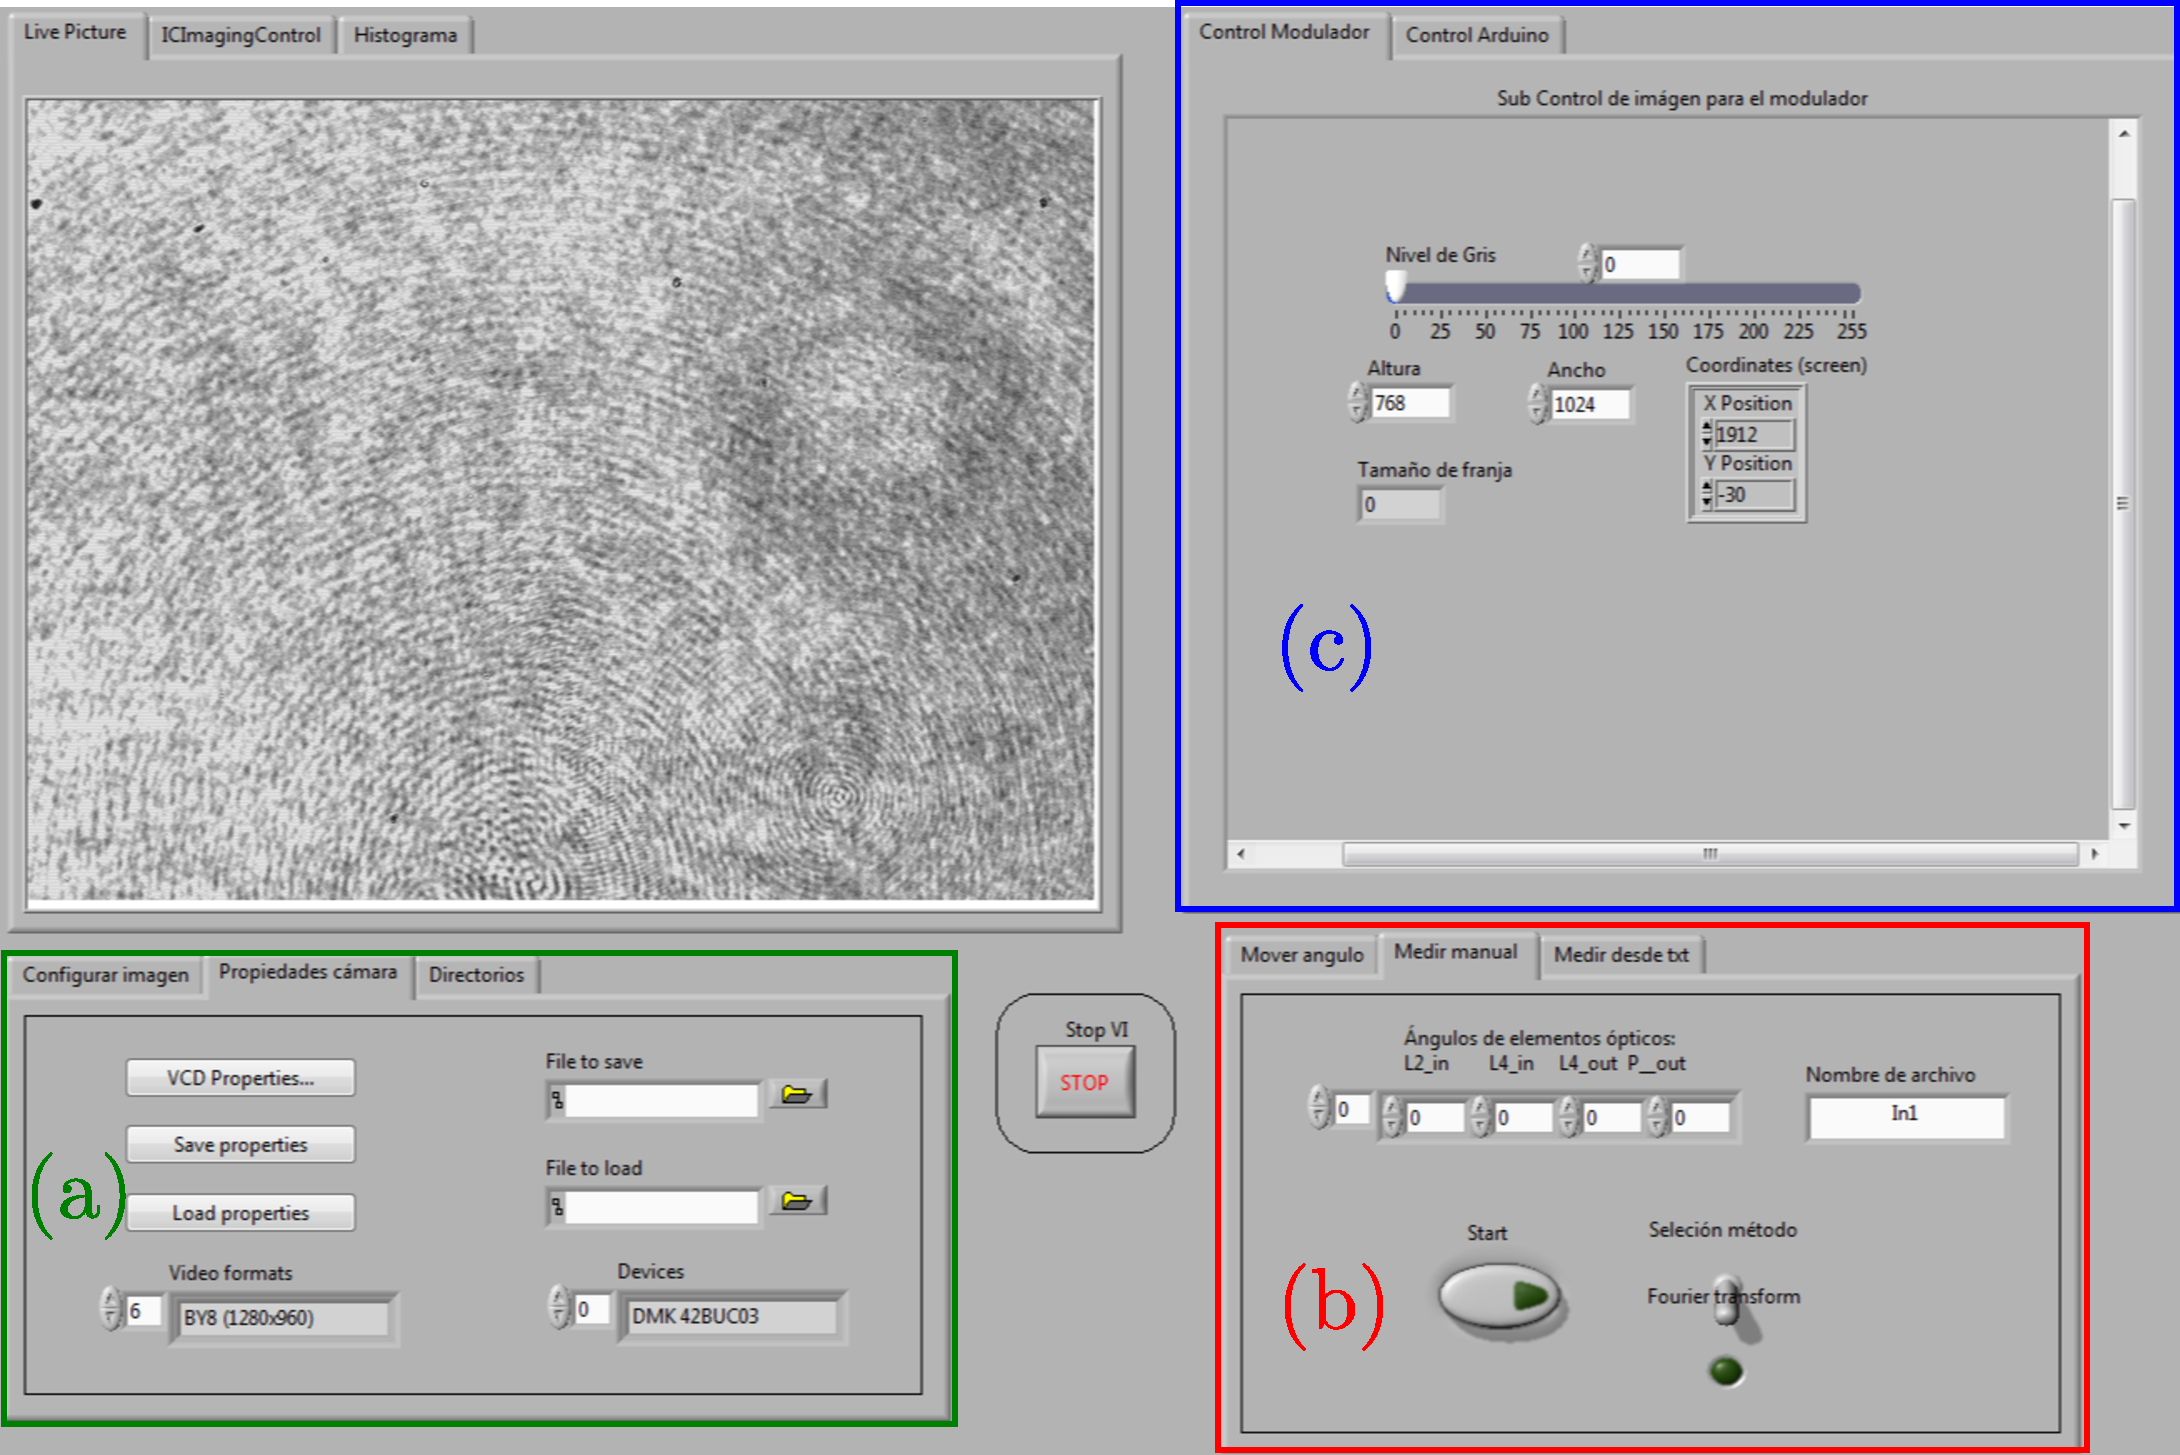
\includegraphics[scale = .4]{SLM_calib2.pdf} 
\caption[Interfaz del programa para toma de medidas 1.]{Otras pestañas
  del Instrumento virtual para toma de medidas. (a) Configuración de
  las propiedades de la cámara, (b) sección para realizar medidas de
  modulación de forma manual y (c) pánel de control para cambiar de
  forma manual las imágenes proyectadas en el SLM para modulación de fase.}
\label{fig:SLM_calib2}
\end{figure}

A continuación, en las siguientes secciones se presenta el código
usado para la programación del microcontrolador Arduino Leonardo, y el
de comunicación entre el computador y el microcontrolador implementado
en el lenguaje Python.
\pagebreak
\section{Programa del Arduino para control de motores de paso}

El programa que se graba en el microcontrolador Arduino permite el
control de hasta 4 motores de paso con rampas de aceleración y
selección de velocidades vía comunicación serial con el computador. 
Los comandos que se pueden enviar al arduino hacen posible consultar,
cambiar o reiniciar la posición y la velocidad de cada motor.
El código se ha alojado en un repositorio en el siguiente vínculo web:
\\
\hspace*{\fill}\href{https://goo.gl/71TdtY}{\textbf{https://goo.gl/71TdtY}}.\hspace*{\fill}\\

% \begin{lstlisting}[style=Arduino]
% #include <AccelStepper.h>
% /*  Program to control two or more stepper motors, with possibility of using acceleration 
%     or deceleration ramps
%     From serial port send:
%      H: To check the status of the serial connection
%      O: To open shutter
%      N: To close shutter
%      D: To query position of current motor
%      C: To change the speed and then send the value 
%      P: To make a given stepper the order to move a given number of steps
%      R: To make a given stepper the order to move at a certain speed
%       S: To stop a stepper that is already running
%       V: To query the speed of a motor that is already running
%   Grupo de Optica Aplicada Universidad EAFIT
%   Author1  Carlos Cuartas, ccuarta1@eafit.edu.co
%   Author2  Santiago Echeverri, sechev14@eafit.edu.co
%   Author3  Camilo Cano, ccanoba@eafit.edu.co
% */
% // Definition of output pins as stepper wires.
% AccelStepper motores[]={AccelStepper (4,5,4,3,2), AccelStepper(4,9,8,7,6), 
%                                         AccelStepper (4,13,12,11,10), AccelStepper (4,A3,A2,A1,A0)};
% int speedIni, paso,n,dummy,engine,rev,cp;    //Definition of variables.
% char parar, vel, cambiar, command;
% float valor,cs;
% const int shutter = A5;
% void setup()
% {  
%   // initialize the LED pin as an output:
%    pinMode(shutter, OUTPUT);   
%    command='\*'; 
%    speedIni = 50;  // Stepper speed in steps per second. 
% // Define maximun speed and acceleration;
% // we recomend using values of 50 (speed) and 20 (acceleration).
%    motores[1].setMaxSpeed(50);   
%    motores[0].setMaxSpeed(50);
%    motores[0].setAcceleration(20);
%    motores[2].setMaxSpeed(50);
%    motores[2].setAcceleration(20);
%    motores[3].setMaxSpeed(50);
%    motores[3].setAcceleration(20);
%    motores[0].setSpeed(50);
%    motores[1].setSpeed(50);
%    motores[2].setSpeed(50);
%    motores[3].setSpeed(50);
%    Serial.begin(9600);	// Start serial port with 9600 baudios of speed.
% }
% float velocidad()   //Funtion to obtain stepper speed.
% {
%   n=steppers(); // Identifies the engine wich you want to get information.
%   valor=motores[n].speed();   // Speed value obtained.
%   return valor;
% }
% int readValue()   // Receives a numerical value at the input of the serial port.
% {
%   // Receive up to 7 bytes,
%   /* http://www.baldengineer.com/blog/2012/07/30/arduino-multi-digit-integers/*/
%    char buffer[] = {' ',' ',' ',' ',' ',' ',' '}; 
%    while (!Serial.available()); // Wait for characters
%    Serial.readBytesUntil('n', buffer, 7);
%    rev = atoi(buffer); //transform string into an int.
%    Serial.println(rev);
%    return rev; 
% }
% int steppers()  // Determines the engine to use.
% {
%   dummy=0;  // Dummy variable, It's use to get into the while.muda
%   while(dummy==0)
%   {
%    engine=readValue(); 
%    if(engine==1)
%    {
%      n=0; //stepper
%      dummy=1;
%      return n;
%    }
%    if(engine==2)
%    {
%      n=1;
%      dummy=1;
%      return n;
%    }
%    if(engine==3)
%    {
%      n=2;
%      dummy=1;
%      return n;
%    }
%    if(engine==4)
%    {
%      n=3;
%      dummy=1;
%      return n;
%    }
%   }
% }
% void loop()  
% {
%   command=Serial.read();  // Wait command.
%    if (command == 'H') // Command to check if we have connexion.
%     {
%       Serial.print('Y');
%       command='\*'; 
%     }
%    if (command == 'Z')
%    {
%      n=steppers();
%      motores[n].setCurrentPosition(0);
%      command='\*';
%    }
%   if (command == 'O') // Command to open shutter.
%     {
%       digitalWrite(shutter, HIGH); 
%      command='\*'; 
%     }
%   if (command == 'N') // Command to close shutter.
%     {
%       digitalWrite(shutter, LOW);  
%       command='\*'; 
%     }         
%   if (command == 'D')
%   {
%     n=steppers();
%     cp=motores[n].currentPosition();
%     Serial.print(cp);
%     command='\*'; 
%   }
% // If the command is C (Change), is because you want to change the stepper speed.
%   if(command =='C')  
%   {
%     speedIni = readValue();
% //Sets the speed, by default it starts with a speed of 50 steps / second.
%       motores[0].setSpeed(speedIni);  
%       motores[1].setSpeed(speedIni);
%       motores[2].setSpeed(speedIni); 
%       motores[3].setSpeed(speedIni);
% //Sets the speed, by default it starts with a speed of 50 steps / second.
%       motores[0].setMaxSpeed(speedIni);  
%       motores[1].setMaxSpeed(speedIni);
%       motores[2].setMaxSpeed(speedIni); 
%       motores[3].setMaxSpeed(speedIni);
%       command='\*'; 
%   }
% // If the command is P (Pasos), then enter the engine you wnat to move and number of steps.
%   if(command =='P')   
%   {
%     n=steppers();
%     paso=readValue();
%     motores[n].moveTo(paso);  //Determines the step at which you want to move the engine.
%     while (motores[n].currentPosition() != paso)
%     motores[n].run();   // Move the motor to the desired step.
%     motores[n].stop();  // This is to avoid mistakes in the deceleration
%     if(motores[n].currentPosition() == paso)
%     {
%       Serial.print('F');
%     }
%     command='\*'; 
%   }
%   // If the command is R (Run), the selected motor will move at constant speed.
%   if(command =='R')  
%   {
%     n=steppers();
%     while(command =='R')
%     {
% //Activates the motor.
%       motores[n].runSpeed();  
% //Receives the command to be used while the engine is moving.    
%       parar = Serial.read();  
%       vel = parar; 
%       cambiar = parar; 
% // If the command is V (Velocidad), returns the speed at which the selected motor moves.       
%       if(vel=='V') 
%       {
%         valor = velocidad();
%         Serial.print(valor);
%         vel='c';
%       }
% //If the command is S (stop), the motor stops.     
%       if(parar=='S')  
%       {
%         Serial.print("Pausa");
%         motores[n].stop();  
%         parar='a';  
%         command='\*'; 
%         cambiar ='ab';
%       }
% //If the command is C (Change), is because you want to change the stepper speed.
%       if(cambiar=='C')  
%       {
%         speedIni = readValue();
%         parar='a';
%         command='\*'; 
%         cambiar='ab';
%       }
%     }
%   }
% }
% \end{lstlisting}

\section{Programa de Python para comunicación serial}
\label{sec:python_serial}

El progama de Python para comunicación serial es un script ejecutable
que permite enviar los comandos seriales de operación del Arduino de
forma simple desde una terminal. Se decidió programar esta aplicación
en el lenguaje Python en vez de hacerlo directamente en el lenguaje de
bloques de LabView para para poder distribuir el código de forma libre
y que cualquiera pudiera operar motores stepper desde arduino sin la
necesidad de tener o usar un programa tan grande y pesado como
LabView. Esta implementación puede servir para, en un futuro controlar
los rotadores desde sistemas embebidos como las plataformas de
desarrollo Raspberry Pi.

La librería que contine los programas para comunicación con el arduino
se han alojado en un repositorio de GitHub en el siguiente vínculo:
\\
\hspace*{\fill}\href{https://goo.gl/tYH0Db}{\textbf{https://goo.gl/tYH0Db}}\hspace*{\fill}\\
% \begin{python}
% #!/usr/bin/env python
% """ Library for communication with an Arduino that powers stepper motors
% This implementation is based on Pyhton3

% Contains one class called ArduinoStepper() that enables the comunication to
% the device along with many usefull commands.

% Grupo de Optica Aplicada Universidad EAFIT

% Author1  Santiago Echeverri, sechev14@eafit.edu.co
% Author2  Carlos Cuartas, ccuarta1@eafit.edu.co
% Author3  Camilo Cano, ccanoba@eafit.edu.co

% """
% from optparse import OptionParser
% import serial
% import os
% class ArduinoStepper():
%     """ Class for basic communication with an arduino for stepper motors control
    
%      1. Detect OS and select the appropiate port preffix.
%         Sometimes linux prefix is: ttyUSB and others is ttyACM
%         I still don't know why...
%      2. Loop over a certain number of port names quering for conection status.

%      At this point all the methods are available for sending commands.
%      Then select either run() and a certain ammount of steps as argument 
%      or goTo() and the desired angle to get to.
%     """
%     def __init__(self, tag, port = ''):
%         if port == '':
%             if os.name == "posix":
%                 # portbase = '/dev/ttyACM'
%                 portbase = '/dev/tty.usbmodem'
%             else:
%                 portbase = 'COM'
    
%             for i in range(100):
%                 try:
%                     self.ser = serial.Serial("%s%d" %(portbase, i),
%                                              baudrate=9600,
%                                              bytesize=8,
%                                              stopbits=1,
%                                              parity=serial.PARITY_NONE,
%                                              timeout=1,
%                                              xonxoff=1)
%                     self.assertConnection()
%                     break
%                 except:
%                     self.ser = None
%                     pass
%         else:
%             self.ser = serial.Serial(port,
%                                              baudrate=9600,
%                                              bytesize=8,
%                                              stopbits=1,
%                                              parity=serial.PARITY_NONE,
%                                              timeout=1,
%                                              xonxoff=1)
%         if self.ser is None:
%             print( "No connection...")
%             return None
%         else:
%             print( "Arduino connected.")
%             self.running = False
%             self.tag = str(tag)
%             pass
%     def sendCom(self, command):
%         self.ser.write(bytes("%s\n" % (command),"UTF-8"))
%         print(self.readReply())
%     def readReply(self):
%         return(self.ser.readline().strip())
%     def assertConnection(self):
%         """ Checks if the arduino is connected"""
%         self.sendCom("H")
%         print(self.ser.readline().strip())
%         assert self.ser.readline().strip() != "Y", "Not connected"
%     def setZero(self):    
%         """ Resets the current position of the motor, so that wherever
%         the motor happens to be right now is considered to be the new 0
%         position. Useful for setting a zero position on a stepper after
%         an initial hardware positioning move. Has the side effect of
%         setting the current motor speed to 0.
        
%         """
%         self.sendCom("Z {0}".format(self.tag))
%         print("Reseting motor {0} to 0.".format(self.tag))
%     def currentStep(self):
%         self.sendCom("D {0}".format(self.tag))
%         sp = self.ser.readline().strip()
%         print("Current step {0}".format(sp))
%         print(self.ser.readline().strip())
%     def run(self,speed):
%         """ Puts a motor in motion at the given speed 
%         Atributes:
%             speed: int speed given in steps per second
%         """
%         self.sendCom("C {0} n R {1}".format(speed, self.tag))
%         print("C {0} n R {1}".format( speed,self.tag))
%         self.running = True
%         print("Running clockwise at {0} steps per second".format(speed))
        
%     def stop(self):
%         """ Stops a running motor """
%         self.sendCom("S")
%         print("Motor stopped")
%         self.running = False
%     def shutter_on(self):    
%         self.sendCom("O")
%     def shutter_off(self):
%         self.sendCom("N")
%     def goTo(self, step):
%         """ Goes to a certain integer step with acceleration ramps

%         A positive value of the argument step implies counter clockwise
%         movement and a negative one counterclockwise. 
%         """
%         if self.running:
%             self.stop()
%         self.running = True
%         self.sendCom("P {0} n {1}".format(self.tag, step))
%         print("Going to step {0}.".format(step))
%     def setSpeed(self, speed):
%         """ Defines speed for goTo 
        
%         Atributes:
%             speed: int speed given in steps per second
%         """
%         self.sendCom("C {0}".format(speed, self.tag))
%         print("C {0}".format( speed,self.tag))
%         self.running = True
%         print("Speed is {0} steps per second".format(speed))
        
%     def getSpeed(self):
%         """ Returns current value of the display
%         This value may be subject to averaging and attenuation.
%         """
%         assert self.running == True, "Only available when in motion"
%         self.sendCom("V")
%         self.sendCom(self.tag)
%         value = self.readReply();
%         try:
%             fvalue = float(value)
%         except:
%             fvalue = None
%         return(fvalue)
       
% if __name__ == "__main__":
%     """ If this file is executed from a terminal the following happens:
    
%     The user has to input an option that describes what is to be done, 
%     at this moment you can choose between:

%     for windows: 
    
%     * Running a certain stepper at a given speed:
%          python.exe ArduinoStepper.py -r 1 -- -100
%       Tells  the motor 1 to run at 100 steps per second counter clockwise
%     * Running a certain stepper to a given step:
%          python.exe ArduinoStepper.py -t 2 -- -400
%       Tells  the motor 2 to go to step -400. 
%     * Stopping a stepper:
%          python.exe ArduinoStepper.py -s 1

%     For mac and linux python.exe is replaced by python.

%     Remember to have a working version of python3.3 with the 
%     pyserial module.
%     """
%     parser = OptionParser(usage="Usage: python3.exe ArduinoStepper.py -s 1 100  ")
%     parser.add_option("-k", "--getSpeed", help = "Returns current stepper speed", type = "int", dest = "samples")
%     parser.add_option("-r", "--run", help = "Puts stepper into motion", type = "int")
%     parser.add_option("-t", "--step", help = "Gets the stepper to a desired step", type = "int")
%     parser.add_option("-s", "--stop", help = "Stops the motor", type = "int")
%     parser.add_option("-o", "--shutterOn", help = "Toggles shutter on", type = "int")
%     parser.add_option("-n", "--shutterOff", help = "Toggles shutter off", type = "int")
%     parser.add_option("-z", "--setZero", help = "Resets current motor counter to zero", type = "int")
%     parser.add_option("-d", "--currentStep", help = "Ask the motor current step", type = "int")
%     parser.add_option("-v", "--setSpeed", help = "Defines speed for function goTo", type = "int")
%     options, args = parser.parse_args()
%     comPort = "COM5"
    
%     if options.run != None:       
%         stepper = ArduinoStepper(options.run, port = comPort)
%         stepper.run(args[0])
%         stepper.ser.close()
%     if options.setSpeed != None:
%         stepper = ArduinoStepper(options.setSpeed, port = comPort)
%         stepper.setSpeed(args[0])
%         stepper.ser.close()
%     if options.setZero != None:
%         stepper = ArduinoStepper(options.setZero, port = comPort)
%         stepper.setZero()
%         stepper.ser.close()
%     if options.currentStep != None:
%         stepper = ArduinoStepper(options.currentStep, port = comPort)
%         stepper.currentStep()
%         stepper.ser.close()
%     if options.stop != None:
%         stepper = ArduinoStepper(options.run, port = comPort)
%         stepper.stop()
%         stepper.ser.close()
%     if options.shutterOn != None:
%         stepper = ArduinoStepper(options.shutterOn, port = comPort)
%         stepper.shutter_on()
%         stepper.ser.close()
%     if options.shutterOff != None:
%         stepper = ArduinoStepper(options.shutterOff, port = comPort)
%         stepper.shutter_off()
%         stepper.ser.close()
%     if options.step != None:
%         stepper = ArduinoStepper(options.step, port = comPort)
%         stepper.goTo(args[0])
%         confirmation = stepper.readReply()
%         while confirmation != b'F':
%             confirmation = stepper.readReply()
%         print(confirmation)
%         stepper.ser.close()
% \end{python}



